\section{FT Model}
\label{sec:FTModel}

This model is designed to read from file the structure of the FT and to import such Boolean logic structure as a RAVEN model.
The FT must be specified in a specific format: the OpenPSA format (\href{<url>}{https://github.com/open-psa}). 
As an example, the FT of Fig.~\ref{fig:FT} is translated in the OpenPSA as shown below:

\begin{lstlisting}[style=XML,morekeywords={anAttribute},caption=FT in OpenPSA format., label=lst:FTModel]
<opsa-mef>
    <define-fault-tree name="FT">
        <define-gate name="TOP">
            <or>
                <gate name="G1"/>
                <gate name="G2"/>
                <gate name="G3"/>
            </or>
        </define-gate>
        <define-component name="A">
            <define-gate name="G1">
                <and>
                    <basic-event name="BE1"/>
                    <basic-event name="BE2"/>
                </and>
            </define-gate>
            <define-gate name="G2">
                <and>
                    <basic-event name="BE1"/>
                    <basic-event name="BE3"/>
                </and>
            </define-gate>
            <define-basic-event name="BE1">
                <float value="1.2e-3"/>
            </define-basic-event>
            <define-component name="B">
                <define-basic-event name="BE2">
                    <float value="2.4e-3"/>
                </define-basic-event>
                <define-basic-event name="BE3">
                    <float value="5.2e-3"/>
                </define-basic-event>
            </define-component>
        </define-component>
        <define-component name="C">
            <define-gate name="G3">
                <and>
                    <basic-event name="BE1"/>
                    <basic-event name="BE4"/>
                </and>
            </define-gate>
            <define-basic-event name="BE4">
                <float value="1.6e-3"/>
            </define-basic-event>
        </define-component>
    </define-fault-tree>
</opsa-mef>
\end{lstlisting} 

\begin{figure}
    \centering
    \centerline{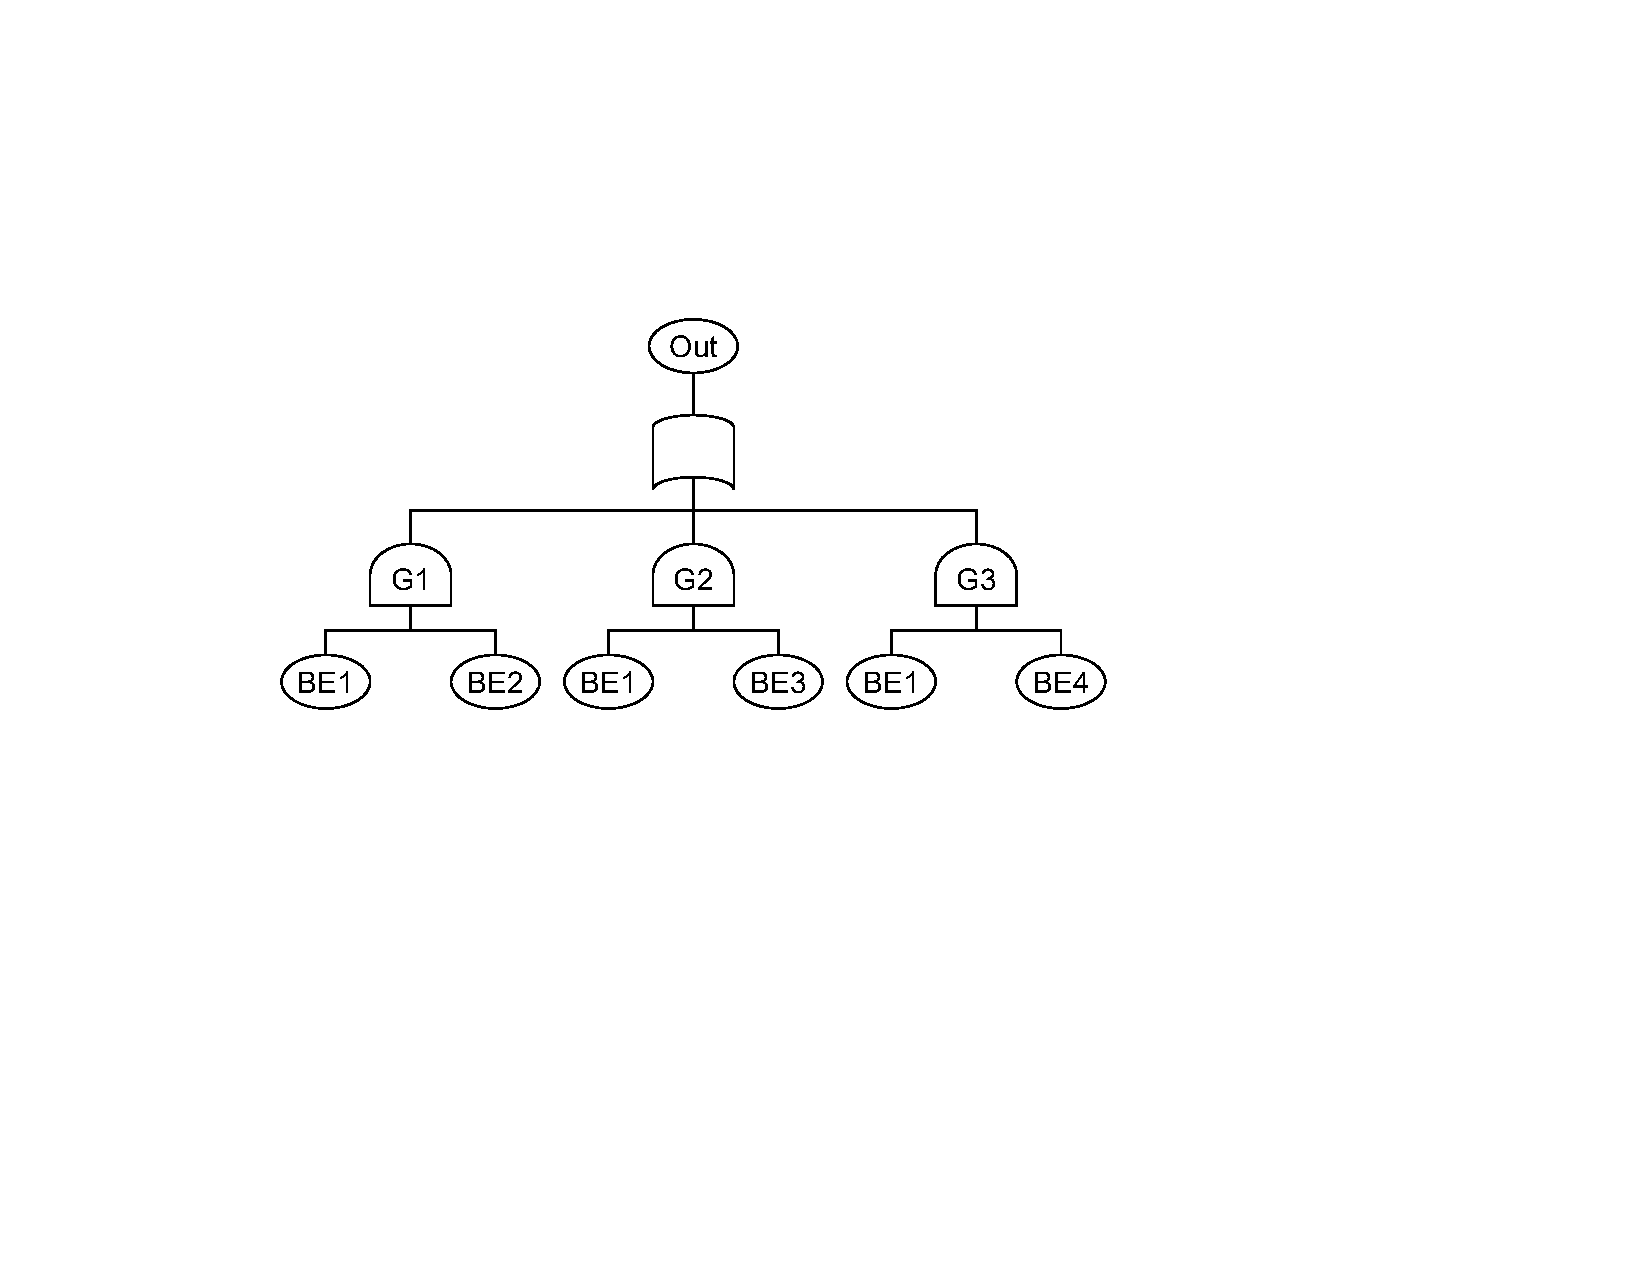
\includegraphics[scale=0.5]{FT.pdf}} 
    \caption{Example of FT.}
    \label{fig:FT}
\end{figure}

The FT of Fig.~\ref{fig:FT} and defined in Listing~\ref{lst:FTModel} can be defined in the RAVEN input file as follows:

\begin{lstlisting}[style=XML,morekeywords={anAttribute},caption=FT model input example., label=lst:FT_InputExample]
  <Models> 
    ...
    <ExternalModel name="FT" subType="FTModel">
      <variables>
        statusBE1,statusBE2,statusBE3,statusBE4,TOP
      </variables>
      <topEvents>TOP</topEvents>
      <map var="statusBE1">BE1</map>
      <map var="statusBE2">BE2</map>
      <map var="statusBE3">BE3</map>
      <map var="statusBE4">BE4</map>
    </ExternalModel>
    ...
  </Models>
\end{lstlisting}

All the specifications of the FT model are given in the 
\xmlNode{ExternalModel} block. 
Inside the \xmlNode{ExternalModel} block, the XML
nodes that belong to this models are:
\begin{itemize}
  \item  \xmlNode{variables}, \xmlDesc{string, required parameter}, a list containing the names of both the input and output variables of the model
  \item  \xmlNode{topEvents},\xmlDesc{string, required parameter}, the name of the alias Top Event
  \item  \xmlNode{map},\xmlDesc{string, required parameter}, the name ID of the FT basic events
	  \begin{itemize}
	    \item \xmlAttr{var}, \xmlDesc{required string attribute}, the ALIAS name ID of the FT basic events
	  \end{itemize}
\end{itemize}

Provided this definition, the FT model of Fig.~\ref{fig:ET} and described in Listing~\ref{lst:ETmodel}, 
the resulting model in RAVEN is characterized by these variables:
\begin{itemize}
	\item Input variables: statusBE1, statusBE2, statusBE3, statusBE4
	\item Output variable: TOP
\end{itemize}

\subsection{FT model reference tests}
\begin{itemize}
	\item test\_FTmodel.xml
	\item test\_FTmodel\_TD.xml
\end{itemize}
